\scanpage{64}\mspage{63}
of $F$, and those of $A$. Moreover, $F$ is the disjoint direct sum of its connected components, i.e. $F=\mathop{\mathrm{Sup}}\limits_i F_i$, the connected components $F_i$ pairwise disjoint\ldots .

% slanted
\margin{\uline{NB} In all this, we do not need $C_3$}

\uline{Connected components of \deleted{$\mathcal F$}the \unsure{country|country} $\mathcal F$.}

Let $M=\coprod_{i\in I}M_i$ be the decomposition of $M$ into connected components.

For every figure $F$, set
\[
F_i=\mathop{\mathrm{Sup}}\limits_{X\in M_i\cap M_{\leq F}}X
\]
% slanted
\margin{We call $F_i$ the \deleted{\unsure{$F_i$}} $i$-component of $F$, or the trace of $F$ on $M_i$ (or on $\mathcal F_i$)}

Then $F$ is the direct sum of the $F_i$, \deleted{and \unsure{?}} If $F$ is of finite type \inserted{(or $I=\pi_0(M)$ finite!)} then all the $F_i$ except a finite number \unsure{are|\deleted{are}} $\varnothing$.
\margin{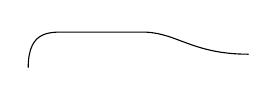
\begin{tikzpicture}[x=1cm,y=1cm]\draw[thin] (0,-.45) .. controls (0,.05) and (.3,0) .. (.55,0) -- (1.5,0) .. controls (1.9,-.02) and (2.1,-.28) .. (2.8,-.28);\end{tikzpicture}}

\deleted{\unsure{Let us write down|Conversely}} Let $\mathcal F_i$ be the set of $F\in\mathcal F$ such that $\overline F\subset M_i$. Then \deleted{\unsure{if}} $\mathcal F_i$ satisfies the conditions $C1,C2$\deleted{$,C3$} (and $C3$ too, if $\mathcal F$ satisfies it), and $M_i$ is the set of its irreducible objects.

\deleted{and the map}
\diagram{\begin{tikzcd}[ampersand replacement=\&,column sep=large,row sep=small,
execute at end picture={\draw[thin,rounded corners=3pt] (oldfamily.south west) -- (oldfigure.west) -- (oldtail.east) .. controls +(right:5pt) and +(right:6pt) .. (oldtail.north east) -- (oldproduct.south west);}]
|[alias=oldfamily]| \mathcal F \arrow[r] \& |[alias=oldproduct]| \prod\mathcal F_i \\
|[alias=oldfigure]| \deleted{F} \arrow[r,mapsto] \& |[alias=oldtail]| \deleted{(F_i)_{i\in I}\ \text{\unsure{or|where} }F_i\ \text{is the}}
\end{tikzcd}}
If $F\in\mathcal F$, if $F_i$ are its components along the $M_i$, then $\overline{F_i}=\overline F\cap M_i$, $\overline F=\deleted{\coprod}\mathop{\bigcup}\limits_i\overline{F_i}$ (disjoint union)

For fixed $i$, the map $F\longrightarrow F_i$ commutes with \inserted{arbitrary Sup, and with nonempty Inf}
\margin{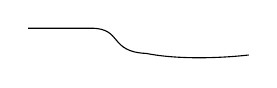
\begin{tikzpicture}[x=1cm,y=1cm]\draw[thin] (0,0) -- (.8,0) .. controls (1.2,0) and (1.02,-.3) .. (1.5,-.32) .. controls (1.9,-.4) and (2.45,-.38) .. (2.8,-.34);\end{tikzpicture}}

The map
\diagram{\begin{tikzcd}[ampersand replacement=\&,column sep=large]
\mathcal F \arrow[r] \& \prod\mathcal F_i \& F \arrow[r,mapsto] \& (F_i)
\end{tikzcd}}
is injective, and the order relation on $\mathcal F$ is induced by the product order
